\documentclass[submit]{harvardml}

\course{CS181-S22}
\assignment{Assignment \#1}
\duedate{7:59pm ET, February 4, 2022} 

\usepackage[OT1]{fontenc}
\usepackage[colorlinks,citecolor=blue,urlcolor=blue]{hyperref}
\usepackage[pdftex]{graphicx}
\usepackage{graphicx}
\usepackage{caption}
\usepackage{fullpage}
\usepackage{soul}
\usepackage{amsmath}
\usepackage{amssymb}
\usepackage{color}
\usepackage{todonotes}
\usepackage{listings}
\usepackage{common}
\usepackage{framed}
\usepackage{physics}
\usepackage{pythonhighlight} 

\usepackage[mmddyyyy,hhmmss]{datetime}

\definecolor{verbgray}{gray}{0.9}

\lstnewenvironment{csv}{
  \lstset{backgroundcolor=\color{verbgray},
  frame=single,
  framerule=0pt,
  basicstyle=\ttfamily,
  columns=fullflexible}}{}
 

\begin{document}
\begin{center}
{\Large Homework 1: Regression}\\
\end{center}

\subsection*{Introduction}
This homework is on different forms of linear regression and focuses
on loss functions, optimizers, and regularization. Linear regression
will be one of the few models that we see that has an analytical
solution.  These problems focus on deriving these solutions and
exploring their properties.

If you find that you are having trouble with the first couple
problems, we recommend going over the fundamentals of linear algebra
and matrix calculus (see links on website).  The relevant parts of the
\href{https://github.com/harvard-ml-courses/cs181-textbook/blob/master/Textbook.pdf}{cs181-textbook notes are Sections 2.1 - 2.7}.  We strongly recommend
reading the textbook before beginning the homework.

    We also encourage you to first read the \href{http://users.isr.ist.utl.pt/~wurmd/Livros/school/Bishop\%20-\%20Pattern\%20Recognition\%20And\%20Machine\%20Learning\%20-\%20Springer\%20\%202006.pdf}{Bishop textbook}, particularly:
Section 2.3 (Properties of Gaussian Distributions), Section 3.1
(Linear Basis Regression), and Section 3.3 (Bayesian Linear
Regression). (Note that our notation is slightly different but the
underlying mathematics remains the same!).

\textbf{Please type your solutions after the corresponding problems using this
\LaTeX\ template, and start each problem on a new page.} You may find
the following introductory resources on \LaTeX\ useful: 
\href{http://www.mjdenny.com/workshops/LaTeX_Intro.pdf}{\LaTeX\ Basics} 
and \href{https://www.overleaf.com/learn/latex/Free_online_introduction_to_LaTeX_(part_1)}{\LaTeX\ tutorial with exercises in Overleaf}

Homeworks will be submitted through Gradescope. You will be added to
the course Gradescope once you join the course Canvas page. If you
haven't received an invitation, contact the course staff through Ed.

\textbf{Please submit the writeup PDF to the Gradescope assignment
  `HW1'.} Remember to assign pages for each question.

\textbf{Please submit your \LaTeX file and code files to the
  Gradescope assignment `HW1 - Supplemental'.} Your files should be
named in the same way as we provide them in the repository,
e.g. \texttt{T1\_P1.py}, etc.


%%%%%%%%%%%%%%%%%%%%%%%%%%%%%%%%%%%%%%%%%%%%%
% Problem 1
%%%%%%%%%%%%%%%%%%%%%%%%%%%%%%%%%%%%%%%%%%%%%

\begin{problem}[Optimizing a Kernel, 15pts]

Kernel-based regression techniques are similar to nearest-neighbor
regressors: rather than fit a parametric model, they predict values
for new data points by interpolating values from existing points in
the training set.  In this problem, we will consider a kernel-based
regressor of the form:
\begin{equation*}
  f(x^*) = \sum_{n} K(x_n,x^*) y_n 
\end{equation*}
where $(x_n,y_n)$ are the training data points, and $K(x,x')$ is a
kernel function that defines the similarity between two inputs $x$ and
$x'$. Assume that each $x_i$ is represented as a column vector, i.e. a
$D$ by 1 vector where $D$ is the number of features for each data
point. A popular choice of kernel is a function that decays as the
distance between the two points increases, such as
\begin{equation*}
  K(x,x') = \exp\left(\frac{-||x-x'||^2_2}{\tau}\right) = \exp\left(\frac{-(x-x')^T (x-x')}{\tau} \right) 
\end{equation*}
where $\tau$ represents the square of the lengthscale (a scalar value).  In this
problem, we will consider optimizing what that (squared) lengthscale
should be.

\begin{enumerate}

\item Let $\{(x_n,y_n)\}_{n=1}^N$ be our training data set.  Suppose
  we are interested in minimizing the residual sum of squares.  Write
  down this loss over the training data $\mcL(W)$ as a function of $\tau$.

  Important: When computing the prediction $f(x_i)$ for a point $x_i$
  in the training set, carefully consider for which points $x'$ you should be including
  the term $K(x_i,x')$ in the sum.

\item Take the derivative of the loss function with respect to $\tau$.
\end{enumerate}

\end{problem}

\newpage

\begin{framed}
\noindent\textbf{Problem 1} (cont.)\\

\begin{enumerate}
\setcounter{enumi}{2}
\item Consider the following data set:
\begin{csv}
  x , y
  0 , 0
  1 , 0.5
  2 , 1
  3 , 2
  4 , 1
  6 , 1.5
  8 , 0.5 
\end{csv}
And the following lengthscales: $\tau=.01$, $\tau=2$, and $\tau=100$.

Write some Python code to compute the loss with respect to each kernel
for the dataset provided above. Which lengthscale does best?  
For this problem, you can use our staff \textbf{script to compare your
  code to a set of staff-written test cases.} This requires, however,
that you use the structure of the starter code provided in
\texttt{T1\_P1.py}. More specific instructions can be found at the top
of the file \texttt{T1\_P1\_Testcases.py}. You may run the test cases
in the command-line using \texttt{python T1\_P1\_TestCases.py}.
\textbf{Note that our set of test cases is not comprehensive: just
  because you pass does not mean your solution is correct! We strongly
  encourage you to write your own test cases and read more about ours
  in the comments of the Python script.}
  
\item Plot the function $(x^*, f(x^*))$ for each of the
  lengthscales above.  You will plot $x^*$ on the x-axis and the
  prediction $f(x^*)$ on the y-axis.  For the test inputs $x^*$, you
  should use an even grid of spacing of $0.1$ between $x^* = 0$ and
  $x^* = 12$.  (Note: it is possible that a test input $x^*$ lands
  right on top of one of the training inputs above.  You can still use
  the formula!) 

  Initial impressions: Briefly describe what happens in each of the
  three cases.  Is what you see consistent with the which lengthscale
  appeared to be numerically best above?  Describe why or why not.

\item Bonus: Code up a gradient descent to optimize the kernel for the
  data set above.
  Start your gradient descent from $\tau=2$. Report on what you
  find.\\\\

  Note: Gradient descent is discussed in Section 3.4 of the
  cs181-textbook notes and Section 5.2.4 of Bishop, and will be
  covered later in the course!

\end{enumerate}
  
\end{framed}  

\newpage

\section{Problem 1}

\subsection{Part 1}

For our training data set $W = \{(x_n, y_n)\}^N_{n=1}$ we want to write down the residual sum of squares loss over the training data $\mcL(W)$ as a function of $\tau$.

The least sum of squares loss for an estimate $\hat{y}$ is given by the following equation.
\begin{equation*}
    \mcL(W) = \frac{1}{2} \sum_{i = 1}^N (y_i - \hat{y_i})^2
\end{equation*}
From the question, our estimate $\hat{y_i}$ is given by the following equation:
\begin{equation*}
    \hat{y_i} = f(x^*) = \sum_{n = 1}^N K(x_n, x^*)y_n
\end{equation*}
Then plugging this into the equation for the least sum of squares loss gives us:
\begin{equation*}
    \mcL(W) = \frac{1}{2} \sum_{i = 1}^N \left(y_i - \sum_{n=1, i \neq n}^N K(x_n, x_i)y_n\right)^2
\end{equation*}
Note that we include the constraint $i \neq j$ to avoid unfairly impacting our loss. Subbing in our kernel function $K$ as given in the question gives us the following expression for the least sum of squares loss as a function of $\tau$.
\begin{equation*}
    \mcL(W) = \frac{1}{2} \sum_{i=1}^N \left(y_i - \sum_{n=1, i \neq n}^N \exp{\frac{-||x_n - x_i||^2}{\tau}} y_n\right)^2
\end{equation*}

\subsection{Part 2}

We now want to take the derivative of the loss function $\mcL(W)$ with respect to $\tau$.

Let us start with the loss function from Part 1.
\begin{equation*}
    \mcL(W) = \frac{1}{2} \sum_{i=1}^N \left(y_i - \sum_{n=1, i \neq n}^N \exp{\frac{-||x_n - x_i||^2}{\tau}} y_n\right)^2
\end{equation*}
Then taking the derivative with respect to $\tau$ by applying the chain rule gives us:
\begin{equation*}
    \frac{\partial \mcL(W)}{\partial \tau} = \sum_{i=1}^N \left(y_i - \sum_{n=1,i\neq n}^N \exp{\frac{-||x_n - x_i||^2}{\tau}} y_n\right) \left( - \sum_{n=1,i\neq n}^N \left(\frac{||x_n - x_i||}{\tau}\right)^2 \exp{ \frac{-||x_n - x_i||^2}{\tau}} y_n \right)
\end{equation*}

\newpage
\subsection{Part 3}

We want to write Python code to compute the loss with respect to each kernel for the dataset provided in the question for each $\tau \in \{.01, 2, 100\}$.

Let us run the code in \verb+T1_P1.py+. Note that we do not include the $\frac{1}{2}$ in the loss function so that we can pass the provided CS181 test cases.
This computes the following losses for each $\tau$:
\begin{itemize}
    \item $\tau = 0.5$ loss is $8.75$
    \item $\tau = 2$ loss is $3.305$
    \item $\tau = 100$ loss is $120.359$
\end{itemize}

\subsection{Part 4}

We want to plot $(x*, f(x*))$ for each lengthscale $\tau$ from Part 3 and then provide a discussion. After running the code in \verb+T1_P1.py+ we have the following plot of the effect of each lengthscale $\tau$ on our predictions.

\begin{center}
    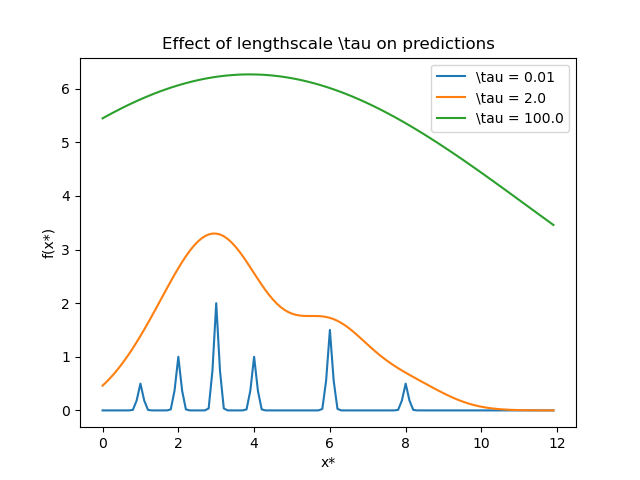
\includegraphics[scale=0.75]{lengthscales.png}
\end{center}

\noindent We now discuss what happens in each of the three values of $\tau$.

As we can see, a $\tau = 0.01$ looks like it is a poor predictor for any new $x^*$ that is not very close to any points in our training data set. Small values of $\tau$ cause our kernel function to return weights close to $0$ for $x^*$ that are not nearly identical to one of our training data points (i.e., $||x_n - x^*||^2$ is small for some $x_n$), meaning that we only sum points in our training data that are very close to the new $x^*$. This causes the spikes in predictions around the points in our training data set, with the regression predicting $0$ otherwise both when interpolating and extrapolating.

In exactly the opposite cause, a $\tau = 100.0$ causes us to use large weights (i.e., close to $1$) for training set data points even if they are far away from our new $x^*$ (i.e., $||x_n - x^*||$ is large for some $x_n$). This is consistent with the figure, which shows how the regression is inflated and smoother, predicting much higher values for new $x^*$ than are in any of our training data when interpolating. Note that because our kernel is not normalized, our predictions are especially large, since we are, in a way, summing all of the points in our data when making predictions for this range of $x^*$.

Finally, $\tau = 2$ seems to strike a good balance. The regression is smooth, slopes with the observed data, and seems to generalize well when interpolating. This ``good fit" is consistent with what we found numerically: $\tau = 2$ had a much lower loss over the training data than the other choices of $\tau$. Like any choice of $\tau$, extrapolating the regression for $x^*$ that are not within the minimum and maximum training data points will eventually cause predictions to go to $0$ for sufficiently large $||x_n - x^*||$.

This result is the same as what we found numerically: a $\tau = 2$ minimized the loss function. This is because a $\tau = 2$ effectively weights nearby points so that the predictions generalize well and are accurate.

\subsection{Part 5 (Bonus)}

We want to code a gradient descent to optimize the kernel for the data set above, starting the gradient descent from $\tau = 2$. If we run the code in \verb+T1_P1.py+, which runs a gradient descent with $10000$ iterations, a learning rate of $0.1$, and a stop threshold of $1\mathrm{e}{-6}$, then we get the following optimal $\tau = 1.708$ and the following regression.
\begin{center}
    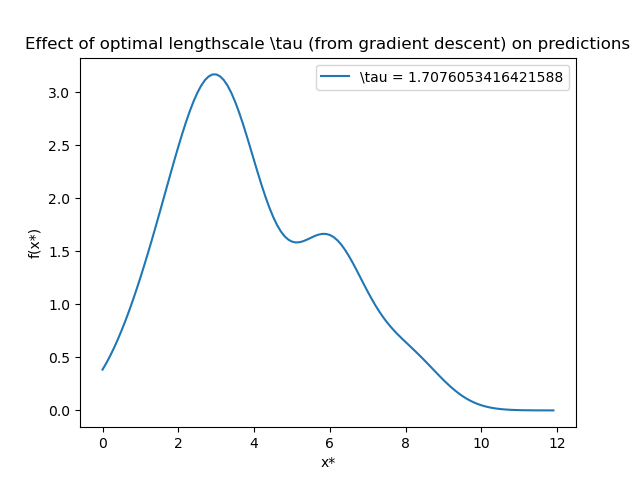
\includegraphics[scale=0.75]{lengthscale-optimal.png}
\end{center}
The loss of this optimal $\tau$ is $3.205$, which is quite close to the loss of $\tau = 2$ from Part 3 and 4. It seems like there are some minor adjustments to the curve that make this $\tau$ more optimal, while still having it be very generalize-able.

\newpage

% %%%%%%%%%%%%%%%%%%%%%%%%%%%%%%%%%%%%%%%%%%%%%
% % Problem 2
% %%%%%%%%%%%%%%%%%%%%%%%%%%%%%%%%%%%%%%%%%%%%%

\begin{problem}[Kernels and kNN, 10pts]

Now, let us compare the kernel-based approach to an approach based on
nearest-neighbors.  Recall that kNN uses a predictor of the form
  \begin{equation*}
    f(x^*) = \frac{1}{k} \sum_n y_n \mathbb{I}(x_n \texttt{ is one of k-closest to } x^*)
  \end{equation*}

\noindent where $\mathbb{I}$ is an indicator variable. For this problem, you will use the \textbf{same dataset and kernel as in Problem 1}.


For this problem, you can use our staff \textbf{script to compare your code to a set of staff-written test cases.} This requires, however, that you use the structure of the starter code provided in \texttt{T1\_P2.py}. More specific instructions can be found at the top of the file \texttt{T1\_P2\_Testcases.py}. You may run the test cases in the command-line using \texttt{python T1\_P2\_TestCases.py}.
\textbf{Note that our set of test cases is not comprehensive: just because you pass does not mean your solution is correct! We strongly encourage you to write your own test cases and read more about ours in the comments of the Python script.}

\vspace{0.5cm}
\noindent\emph{Make sure to include all required plots in your PDF.}


\begin{enumerate}

\item Implement kNN for $k=\{1, 3, N-1\}$ where N is the size of the dataset, then plot the results for each $k$. To find the distance between points, use the kernel function from Problem 1 with lengthscale $\tau=1$. 

As before, you will plot $x^*$ on the x-axis and the prediction $f(x^*)$ on the y-axis.  For the test inputs $x^*$, you should use an even grid of spacing of $0.1$ between $x^* = 0$ and $x^* = 12$.  (Like in Problem 1, if a test point lies on top of a training input, use the formula without excluding that training input.)
  
  You may choose to use some starter Python code to create your plots
  provided in \verb|T1_P2.py|.  Please \textbf{write your own
    implementation of kNN} for full credit.  Do not use external
  libraries to find nearest neighbors.
  
\item Describe what you see: What is the behavior of the functions in
  these three plots?  How does it compare to the behavior of the
  functions in the three plots from Problem 1?  Are there situations
  in which kNN and kernel-based regression interpolate similarly?
  Extrapolate similarly?  Based on what you see, do you believe there
  exist some values of $k$ and $\tau$ for which the kNN and kernel-based regressors produce the exact same classifier (ie. given \textit{any} point $x$, the two regressors will produce the same prediction $f(x)$)? Explain your answer.
  
\item Why did we not vary $\tau$ for the kNN approach?

\end{enumerate}

\end{problem}

\newpage

%%%%%%%%%%%%%%%%%%%%%%%%%%%%%%%%%%%%%%%%%%
\section{Problem 2}

\subsection{Part 1}
We want to implement kNN for $k = \{1, 3, N-1\}$, then plot the results for each $k$ using the kernel function from Problem 1 and $\tau = 1$ to find the distance between points.

After running the code in \verb+T1_P2.py+, we get the following three plots.

\begin{figure}[h]
\begin{tabular}{ccc}
    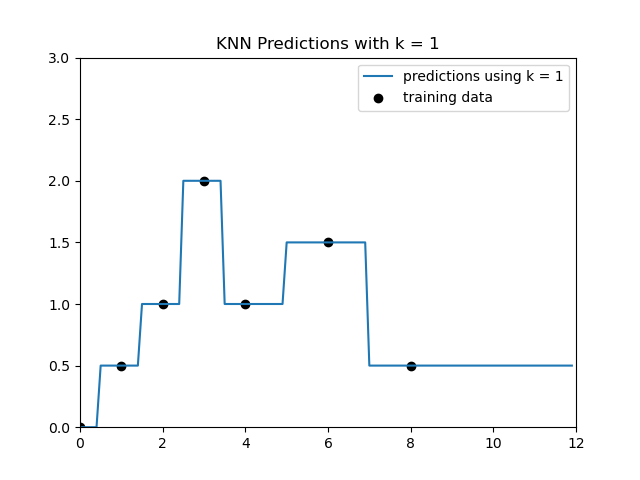
\includegraphics[width=0.5\textwidth]{k1.png} & 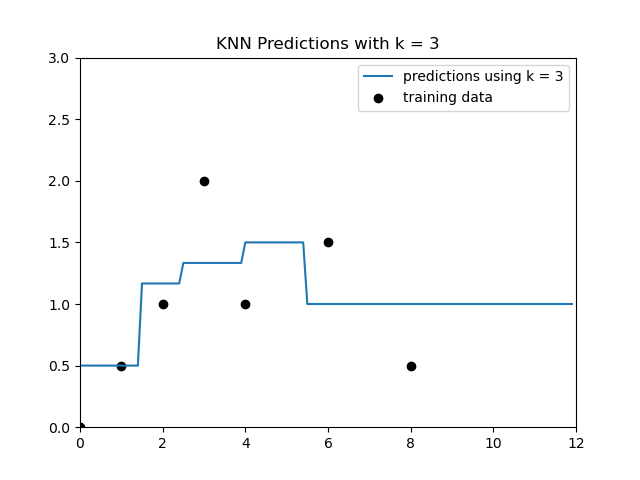
\includegraphics[width=0.5\textwidth]{k3.png} \\ \multicolumn{2}{c}{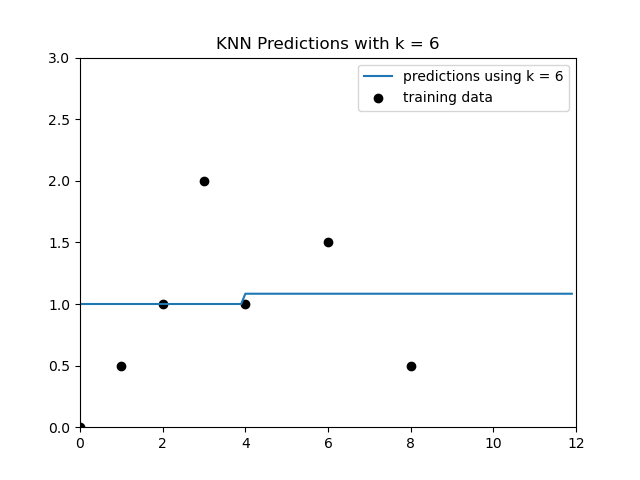
\includegraphics[width=0.5\textwidth]{k6.png}}
\end{tabular}
\end{figure}

\subsection{Part 2}

First, let us describe the behavior of the functions in the three plots. A value of $k = 1$ only considers the training data point that is closest to the new $x^*$, causing a ``step-like" effect where predictions for $x^*$ are equal to the closest training data point, until a new closest point is reached. A value of $k = 3$ is smoother: since we consider the three closest training data points, our regression seems to be more of an average between the three closest points. Finally, the $k = 6$ case prediction is basically an average of all the training data since $k = 6$ and there are $7$ training data points, with a step around the median of the data.

The behavior of these functions is generally different than from Problem 1. The $k = 1$ function does seem to interpolate somewhat similarly to the $\tau = 0.01$ function in the sense that we return predictions that are identical to the closest training data point for new $x^*$ that are close to a training data point, but the behavior when interpolating for new $x^*$ that are farther away from any training data points is different because for the kernel we use a weight rather than an indicator variable and so return $0$ instead of still returning the value of the closest point. The $k = 3$ case also seems to interpolate similarly to the $\tau = 2.0$ case: both are smoother and seem to average the nearest points to a greater extent than the other functions. All of the kNN functions extrapolate differently than the kernel-based regression. This is similarly due to the fact that kNN uses an indicator variable rather than weights: as the distance between the new $x^*$ and the closest data point increases, eventually the kernel will return $0$, whereas the kNN method continues to return the value of the closest data points.

Based on what I see, there is no value of $k$ and $\tau$ for which kNN and kernel-based regressors produce the exact same classifier. This can be seen in the differences in how each method extrapolates: since kNN uses weights, the predictions eventually go to $0$ as the distance increases between the new $x^*$ and any of the training data points, whereas kNN will continue to return the values of the closest data points.

\subsection{Part 3}
We did not vary $\tau$ for the kNN approach because varying $\tau$ does not affect the relative values of closeness for the points in our training data to our new point $x^*$, and so thus does not affect our regression. Since kNN uses an indicator variable to choose the $k$-closest points, our prediction only considers which of the training data points are among the $k$-closest points, not how close they actually are to $x^*$. Thus we will always have the same set of $k$-closest points for any $\tau$, and so varying $\tau$ does not affect our regression.

\newpage 

%%%%%%%%%%%%%%%%%%%%%%%%%%%%%%%%%%%%%%%%%%%%%
% Problem 3
%%%%%%%%%%%%%%%%%%%%%%%%%%%%%%%%%%%%%%%%%%%%%

\begin{problem}[Deriving Linear Regression, 10pts]

  The solution for the least squares linear regressions ``looks'' kind
  of like a ratio of covariance and variance terms.  In this problem,
  we will make that connection more explicit. \\

  \noindent Let us assume that our data are tuples of scalars $(x,y)$ that are
  described by some joint distribution $p(x,y)$.  For clarification, the joint distribution $p(x,y)$ is just another way of saying the ``joint PDF'' $f(x,y)$, which may be more familiar to those who have taken Stat 110, or equivalent. \\
  
  \noindent We will consider the process of fitting these data from this distribution with the best linear model
  possible, that is a linear model of the form $\hat{y} = wx$ that
  minimizes the expected squared loss $E_{x,y}[ ( y - \hat{y} )^2
  ]$.\\

\noindent \emph{Notes:} The notation $E_{x, y}$ indicates an
expectation taken over the joint distribution $p(x,y)$.  Since $x$ and
$y$ are scalars, $w$ is also a scalar.
  
  \begin{enumerate}

  \item Derive an expression for the optimal $w$, that is, the $w$
    that minimizes the expected squared loss above.  You should leave
    your answer in terms of moments of the distribution, e.g. terms
    like $E_x[x]$, $E_x[x^2]$, $E_y[y]$, $E_y[y^2]$, $E_{x,y}[xy]$
    etc.

\item Provide unbiased and consistent formulas to estimate $E_{x, y}[yx]$
 and $E_x[x^2]$ given observed data $\{(x_n,y_n)\}_{n=1}^N$.

\item In general, moment terms like $E_{x, y}[yx]$, $E_{x, y}[x^2]$,
  $E_{x, y}[yx^3]$, $E_{x, y}[\frac{x}{y}]$, etc. can easily be
  estimated from the data (like you did above).  If you substitute in
  these empirical moments, how does your expression for the optimal
  $w^*$ in this problem compare with the optimal $w^*$ that we see in
  Section 2.6 of the cs181-textbook?

\item Many common probabilistic linear regression models assume that
  variables x and y are jointly Gaussian.  Did any of your above
  derivations rely on the assumption that x and y are jointly
  Gaussian?  Why or why not?
    
\end{enumerate}

\end{problem}

\newpage

\section{Problem 3}

\subsection{Part 1}
We want to derive an expression for the optimal $w$, leaving our answer in terms of moments of the distribution.
The optimal $w$ minimizes the expected squared loss, which is given by the following expression.
\begin{equation*}
    E_{x,y}[(y - \hat{y})^2]
\end{equation*}
We can expand this expression, sub-in $\hat{y} = w x$, and apply linearity of expectation.
\begin{align*}
    E_{x,y}[(y - \hat{y})^2] &= E_{x,y}[y^2 - 2\hat{y}y + \hat{y}^2]\\
    &= E_{x,y}[y^2 - 2 w x y + w^2 x^2]\\
    &= E_{x,y}[y^2] - 2 w E_{x,y}[x y] + w^2 E_{x,y}[x^2]
\end{align*}
Notice that $E_{x,y}[x^2] = E_x[x^2]$ and $E_{x,y}[y^2] = E_y[y^2]$. And so we can further simplify this expression.
\begin{align*}
    E_{x,y}[(y - \hat{y})^2] &= E_{y}[y^2] - 2 w E_{x,y}[x y] + w^2 E_{x}[x^2]
\end{align*}
Then to find the optimal $w$ we can then take the derivative of this expression with respect to $w$.
\begin{align*}
    \frac{\partial E_{x,y}[(y - \hat{y})^2]}{\partial w} &= 2 E_{x,y}[x y] + 2 w E_{x}[x^2]
\end{align*}
The optimal $w$ occurs when this expression is equal to $0$. Setting the left-hand side to $0$ and simplifying yields an expression for the optimal $w$.
\begin{align*}
    0 &= 2 E_{x,y}[x y] + 2 w E_{x}[x^2]\\
    w &= \frac{E_{x,y}[x y]}{E_{x}[x^2]}
\end{align*}

\subsection{Part 2}
We want to provide unbiased and consistent formulas to estimate $E_{x,y}[y x]$ and $E_x[x^2]$ given observed data $\{(x_n,y_n)\}_{n=1}^N$. We can use the sample mean for each expression, which is consistent and unbiased.
\begin{equation*}
    E_{x,y}[y x] = \frac{1}{N} \sum_{n=1}^N y_n x_n\ , \ E_x[x^2] = \frac{1}{N} \sum_{n=1}^N x_n^2
\end{equation*}

\subsection{Part 3}

We want to compare how our expression for the optimal $w^*$ from Part 2 compares to the optimal $w^*$ from the textbook.
Let us write the expression for the optimal $w^*$ from the textbook.
\begin{equation*}
    \vb{w}^* = (\vb{X}^T \vb{X})^{-1} \vb{X}^T \vb{y}
\end{equation*}
Since our data are tuples of scalars, we know that $\vb{X}$ is a $N \times 1$ vector and $\vb{y}$ is a $N \times 1$ vector. We can write $\vb{X}$ and $\vb{y}$ as follows.
\begin{equation*}
    \vb{X} =
        \begin{bmatrix}
            x_1\\
            \vdots\\
            x_N
        \end{bmatrix}
    \ , \
    \vb{y} = 
        \begin{bmatrix}
            y_1\\
            \vdots\\
            y_N
        \end{bmatrix}
\end{equation*}
We can write $\vb{X}^T \vb{X}$ as the following.
\begin{equation*}
    \vb{X}^T \vb{X} = x_1 x_1 + \cdots + x_N x_N = \sum_{n = 1}^N x_n^2
\end{equation*}
Then taking the inverse yields the expression below.
\begin{equation*}
    (\vb{X}^T \vb{X})^{-1} = \frac{1}{\sum_{n = 1}^N x_n^2}
\end{equation*}
We can also expand $\vb{X}^T \vb{y}$.
\begin{equation*}
    \vb{X}^T \vb{y} = x_1 y_1 + \cdots + x_N y_N = \sum_{n=1}^N x_n y_n
\end{equation*}
Finally, we sub these into the optimal expression for $w*$.
\begin{equation*}
    w^* = (\vb{X}^T \vb{X})^{-1} \vb{X}^T \vb{y} = \frac{\sum_{n=1}^N x_n y_n}{\sum_{n = 1}^N x_n^2}
\end{equation*}
This expression identically matches our expression that we obtained for the optimal $w^*$ in Part 1!

\subsection{Part 4}
Our derivations did not rely on the assumption that $x,y$ are jointly Gaussian. We did not use any of the properties of the Gaussian distribution in our derivations, we only used the properties of expectation, which are not specific to any particular distribution.

\newpage

% %%%%%%%%%%%%%%%%%%%%%%%%%%%%%%%%%%%%%%%%%%%%%
% % Problem 4
% %%%%%%%%%%%%%%%%%%%%%%%%%%%%%%%%%%%%%%%%%%%%%

\begin{problem}[Modeling Changes in Republicans and Sunspots, 15pts]
  
 The objective of this problem is to learn about linear regression
 with basis functions by modeling the number of Republicans in the
 Senate. The file \verb|data/year-sunspots-republicans.csv| contains the
 data you will use for this problem.  It has three columns.  The first
 one is an integer that indicates the year.  The second is the number
 of Sunspots observed in that year.  The third is the number of Republicans in the Senate for that year.
 The data file looks like this:
 \begin{csv}
Year,Sunspot_Count,Republican_Count
1960,112.3,36
1962,37.6,34
1964,10.2,32
1966,47.0,36
\end{csv}

You can see scatterplots of the data in the figures below.  The horizontal axis is the Year, and the vertical axis is the Number of Republicans and the Number of Sunspots, respectively.

\begin{center}
\includegraphics[width=.5\textwidth]{data/year-republicans}
\end{center}

\begin{center}
\includegraphics[width=.5\textwidth]{data/year-sunspots}
\end{center}

(Data Source: \url{http://www.realclimate.org/data/senators_sunspots.txt})\\
\vspace{-5mm}


\vspace{0.5cm}
\noindent\emph{Make sure to include all required plots in your PDF.}

\begin{enumerate}

\item In this problem you will implement ordinary least squares
  regression using 4 different basis functions for \textbf{Year
    (x-axis)} v. \textbf{Number of Republicans in the Senate
    (y-axis)}. Some starter Python code that implements simple linear
  regression is provided in \verb|T1_P4.py|.

  Note: The numbers in the \emph{Year} column are large (between $1960$ and $2006$), especially when raised to various powers. To avoid numerical instability due to ill-conditioned matrices in most numerical computing systems, we will scale the data first: specifically, we will scale all ``year'' inputs by subtracting $1960$ and then dividing by $40$. Similarly, to avoid numerical instability with numbers in the \emph{Sunspot\_Count} column, we will also scale the data first by dividing all ``sunspot count'' inputs by $20$. Both of these scaling procedures have already been implemented in lines $65-69$ of the starter code in \verb|T1_P4.py|. Please do \emph{not} change these lines!

First, plot the data and regression lines for each of the following sets of basis functions, and include
the generated plot as an image in your submission PDF. You will therefore make 4 total plots:
\begin{enumerate}
	\item[(a)] $\phi_j(x) = x^j$ for $j=1, \ldots, 5$\\
    ie, use basis $y = a_1 x^1 + a_2 x^2 + a_3 x^3 + a_4 x^4 + a_5 x^5$ for some constants $\{a_1, ..., a_5\}$. 
    \item[(b)] $\phi_j(x) = \exp{\frac{-(x-\mu_j)^2}{25}}$ for $\mu_j=1960, 1965, 1970, 1975, \ldots 2010$
	\item[(c)] $\phi_j(x) = \cos(x / j)$ for $j=1, \ldots, 5$
	\item[(d)] $\phi_j(x) = \cos(x / j)$ for $j=1, \ldots, 25$
\end{enumerate}
\vspace{-2mm}


{\footnotesize * Note: Please make sure to add a bias term for all your basis functions above in your implementation of the \verb|make_basis| function in \verb|T1_P4.py|.}
  
Second, for each plot include the residual sum of squares error. Submit the generated plot and residual sum-of-squares error for each basis in your LaTeX write-up.
\end{enumerate}

\end{problem}

\begin{framed}
\noindent\textbf{Problem 4} (cont.)\\
\begin{enumerate}
\setcounter{enumi}{1}
\item Repeat the same exact process as above but for \textbf{Number of Sunspots (x-axis)} v. \textbf{Number of Republicans in the Senate (y-axis)}. 
Now, however, only use data from before 1985, and only use basis functions (a), (c), and (d) -- ignore basis (b). You will therefore make 3 total plots. For each plot make sure to also include the residual sum of squares error.



Which of the three bases (a, c, d) provided the "best" fit? \textbf{Choose one}, and keep in mind the generalizability of the model. 

Given the quality of this fit, do you believe that the number of sunspots controls the number of Republicans in the senate (Yes or No)?
\end{enumerate}
\end{framed}

\newpage

%%%%%%%%%%%%%%%%%%%%%%%%%%%%%%%%%%%%%%%%
\section{Problem 4}

\subsection{Part 1}
We want to plot the data and regression lines for the sets of basis functions (a) through (d) for year ($x$-axis) and number of republicans in the senate ($y$-axis), and include the residual sum of squares error.

Running the code in \verb+T1_P4.py+ outputs the plots below for each basis function. The basis function is given in the title of each plot.
\begin{figure}[h]
\begin{tabular}{cc}
    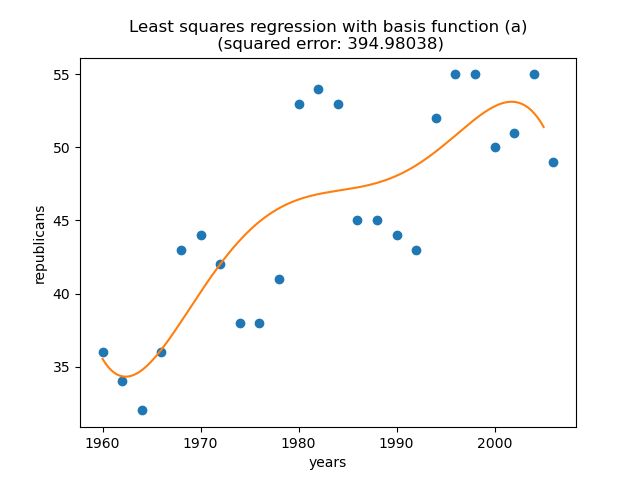
\includegraphics[width=0.5\textwidth]{4-1-a.png} & 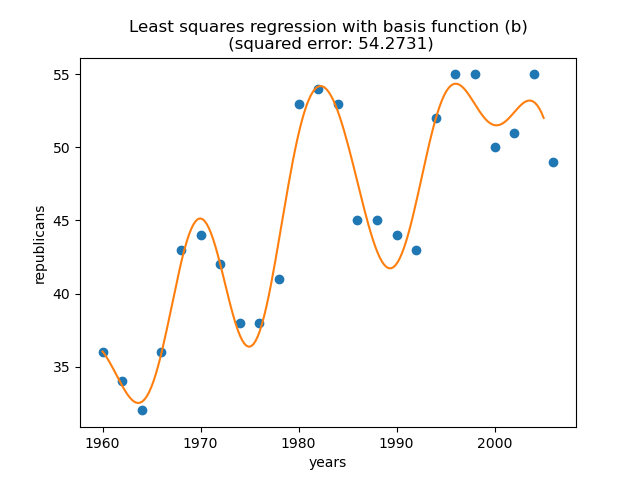
\includegraphics[width=0.5\textwidth]{4-1-b.png} \\
    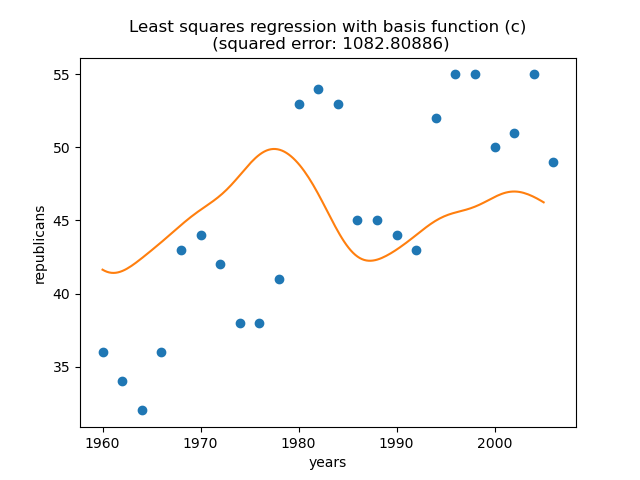
\includegraphics[width=0.5\textwidth]{4-1-c.png} & 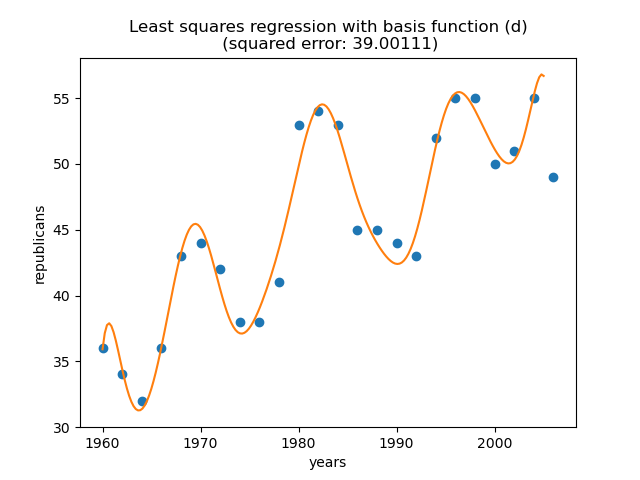
\includegraphics[width=0.5\textwidth]{4-1-d.png} \\
\end{tabular}
\end{figure}

The residual sum of squares error for each basis function is in the title of each plot, but is also given below for convenience.
\begin{itemize}
    \item (a) error is $394.98038$
    \item (b) error is $54.2731$
    \item (c) error is $1082.80886$
    \item (d) error is $39.00111$
\end{itemize}

\newpage

\subsection{Part 2}
We want to plot the data and regression lines for the sets of basis functions (a), (c), and (d) for the number of sunspots ($x$-axis) and the number of republicans in the senate ($y$-axis) for data from before 1985, and include the residual sum of squares error.
Running the code in \verb+T1_P4.py+ outputs the plots below for each basis function. The basis function is given in the title of each plot.
\begin{figure}[h]
\begin{tabular}{cc}
    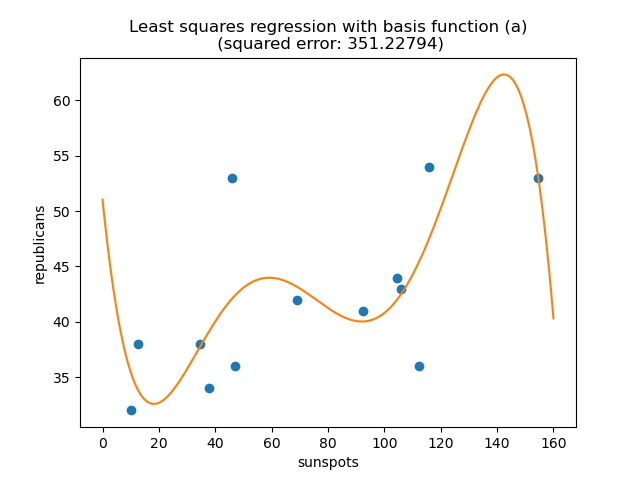
\includegraphics[width=0.5\textwidth]{4-2-a.png} & 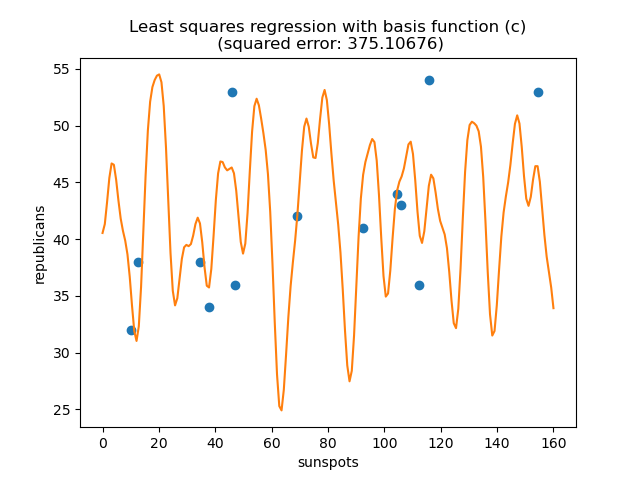
\includegraphics[width=0.5\textwidth]{4-2-c.png} \\
    \multicolumn{2}{c}{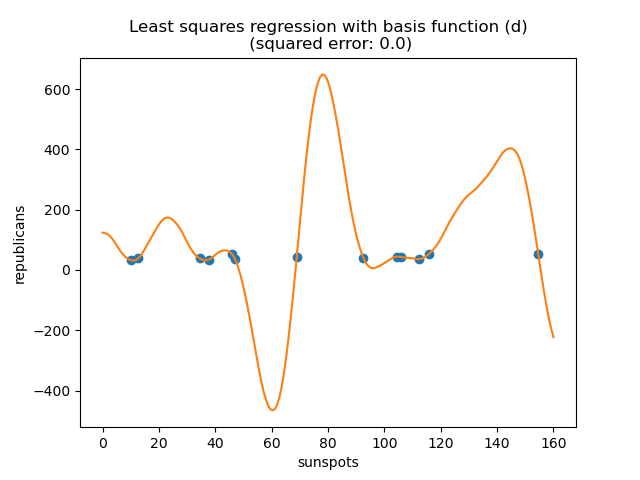
\includegraphics[width=0.5\textwidth]{4-2-d.png}}
\end{tabular}
\end{figure}

The residual sum of squares error for each basis function is in the title of each plot, but is also given below for convenience.
\begin{itemize}
    \item (a) error is $351.22794$
    \item (c) error is $375.10676$
    \item (d) error is $0.0$
\end{itemize}

I think that basis function (a) provides the "best" fit. Basis function (c) is incredibly noisy and sporadic, causing large changes in the $y$-axis over small changes in the $x$-axis that do not seem to fit the data or be generalize-able at all. Basis function (d), despite having a squared error of $0$, looks like it over-fits the data to an extreme and looks like it is not generalize-able. Basis function (a), although having fairly large square error, looks like it fits the data set as well as possible without over-fitting.

No, I do not believe the number of sunspots controls the number of republicans in the senate. The fit of (a), while the best of the three basis functions, is poor, and so I would argue that the number of sunspots does not control the number of republicans in the senate.

%%%%%%%%%%%%%%%%%%%%%%%%%%%%%%%%%%%%%%%%

\newpage
%%%%%%%%%%%%%%%%%%%%%%%%%%%%%%%%%%%%%%%%%%%%%
% Name and Calibration
%%%%%%%%%%%%%%%%%%%%%%%%%%%%%%%%%%%%%%%%%%%%%
\subsection*{Rob Walker}

\subsection*{Collaborators and Resources}
Whom did you work with, and did you use any resources beyond cs181-textbook and your notes?

James Kitch and Julian Schmitt. When working on Problem 1.5 (bonus), I referenced this article: https://www.geeksforgeeks.org/how-to-implement-a-gradient-descent-in-python-to-find-a-local-minimum/ when writing my gradient descent in Python.

\subsection*{Calibration}
Approximately how long did this homework take you to complete (in hours)? 
20 hours

\end{document}